\chapter{Temporal Side Channels I} 

\section{History}
In 1995, When he was 22, Paul Kaucher released a paper called Timing attacks on implementations of Diffie-Helman, RSA, DSS and other systems \cite{kocher1996timing}.

Before it was published, he wrote about it in a mailing list of Cypherpunks\footnote{A cypherpunk is any activist advocating widespread use of strong cryptography and privacy-enhancing technologies as a route to social and political change. Originally communicating through the Cypherpunks electronic mailing list, informal groups aimed to achieve privacy and security through proactive use of cryptography}
which included all sorts of people like mathematicians, photographers, artists anarchists and more.
The attack was first demonstrated in 1997 in a cryptography conference.
And later, in 1998 an academic paper was published describing how to perform the attack.



\section{The Threat Model}
Figure \ref{c1_fig_threat_model} descirbes the Threat Model on an implementation of some secure system.
It is important to mention that we're talking about attacking an implementation, and not the algorithm itself as we consider the algorithm or protocol being examined as completely secure.

\begin{figure}[H]
    \centering
    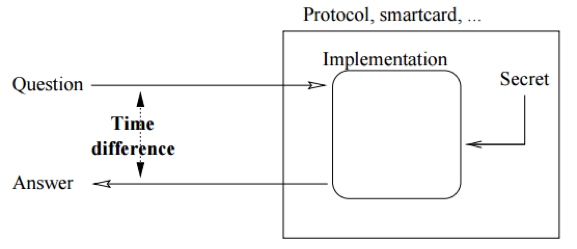
\includegraphics{images/chapter_1/threat_model.png}
    \caption{The Threat Model. Image from JF Dhem1998.
     The attacker can send a message to the implementation and get an answer from it. Also - the attacker is able to measure the time it takes for the implementation to compute the output}
    \label{c1_fig_threat_model}
\end{figure}

\subsection{When is a timing attack even possible?}
\begin{enumerate}
    \item Physical access to the device.
    (for example: Smart card, Crypto wallet, Electronic voting machines)
    \item Sharing a virtual machine with the service
    (for example: Swiping a credit card)
    \item Remote access to a device (access to a device over the network, which may be very noisy and may be rather difficult to implement)
\end{enumerate}

The objective of the attacker to discover the password. And what could the attacker do? The attacker can send unlimited queries and measure their time. Unlimited queries are not so trivial, If you think about it. Some devices can disable themselves after 3 or 4 or 5 periods. This can be a defense \cite{ATM_bruteforce_block}

\section{Timing attack}

\begin{figure}[H]
    \centering
    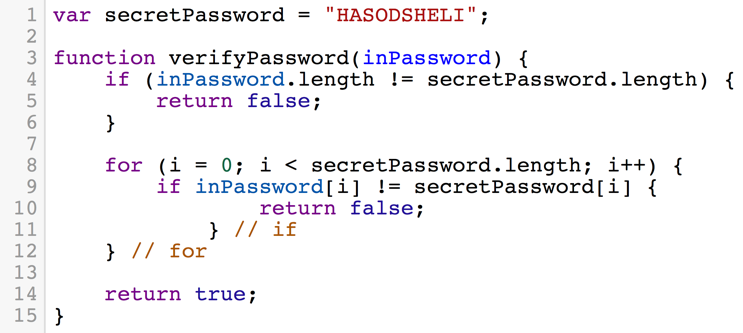
\includegraphics{images/chapter_1/password_check_algo_1.png}
    \caption{A simple and efficient password checking algorithm.
    In line 4 there's a check if there length of the password is the same as the length of the input.
    In line 8 there's an iteration over all of the characters in the }
    \label{c1_fig_pass_check_1}
\end{figure}

Consider the algorithm for password checking as described in figure \ref{c1_fig_pass_check_1}

In a scenario where timing attack is not possible, breaking the password requires the attacker
 to bruteforce the password.
 That is, checking every possible string for one successful attempt.

Let's assume the password is of length 16, if the password only contains english upper-case characters we have 26 possible values for each of the 16 characters in the password.
The first character has 26 possiblites, the second has 26 possiblites and so on. 
So bruteforcing a password like this requries ${26}^{16}$ different attempts, which cannot be completed by any computer in a decent amount of time.
In general, for a password of length $n$ and character range of size $k$,
 breaking the password will take $O({k}^{n})$ attempts.

Now let's consider the scenrio where \textbf{timing attack is possible}. To perform a timing attack,
the attacker takes advantage of the fact that when the program checks for strings equality, the comparison will finish as soon as it finds one character that doesn't match.
Consider the following example where the attacker tries the 3 following attempts and measures
the time it takes for the machine to respond. The attacker tries "AAAA" and measures 0.2ms, then tries "BAAA" and measures 0.5ms lastly tries "CAAA" and measures 0.2ms again.
The attack can be pretty sure that the first character is "B".
Now, checking the whole password does not require iterating of all possible combinations of strings of size $n$. 
All it takes is to iterate over all possible values of each character, say $k$, and repeat that $n$ times.
This results in a total runtime of $k+k+k+\dots = nk = O(n)$

We can now break the password in a reasonable amount of time, even without knowing the 
length of the password we're trying to crack.

\section{Timing Attack Defenses}
After discussing the potential of such attack, we now consider the possible mitigations we can 
implement on our system to prevent such attacks.

\subsection{Mitigation}
We can consider adding a random wait time after checking each one of the characters.
The problem of course is that the whole process of checking a valid process becomes slower.
And of course, if the attacker can perform a lot of measurements on our system, since the noise is random, the attacker would be able to ignore it.


\subsection{Prevention}
The second type of countermeasure is prevention, making sure that our system is completely resistant to timing attacks.

\subsubsection{Prevention Method 1: Padding}
\begin{figure}[H]
    \centering
    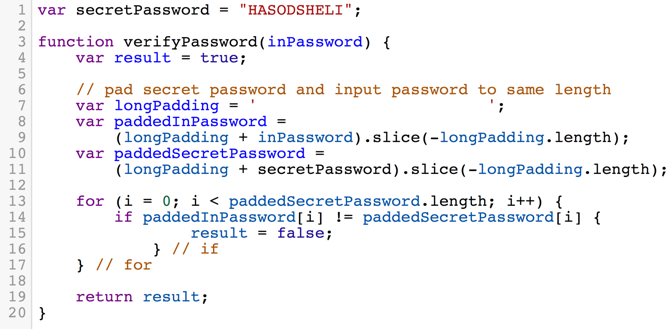
\includegraphics{images/chapter_1/password_check_algo_2.png}
    \caption
    {Prevention method 2, padding the user guess and the secret password to the 
    same length and check all characters even if there's a mismatch in the first character.}
    \label{c1_fig_pass_check_2}
\end{figure}

The first method we examine is to pad the secret password and the user's guess to the same length.
Also - we do not return as soon as we see a character mismatch.
 The code is described in figure 
 \ref{c1_fig_pass_check_2}

The problem with this implementation is that every time there's a character mismatch we execute additional code.
Which is loading the variable \lstinline{result} and writing the value \lstinline{false} to it.
This may seem insignificant in the beginning but actually, this is makes our code \textbf{much more vulnerable than it was before}.
As now the time of it takes for the entire function to complete is linearly dependant on the amount of characters mismatches we have, 
this allows an attacker to perform the same attack from before with no significant changes to his original timing attack.

One might think of a fix which is adding another branch to the \lstinline{if} statement that will do some garbage operation like \lstinline{foo = false}
just so that the attacker might not be able to tell the difference between a match and a mismatch.
The problem with this fix might be that the access time to one variable may be different than the access time to another variable,
and the attacker will be able to tell the difference between them.


\subsection{Prevention Method 2: Hashing}
\begin{figure}[H]
    
    % \centering
    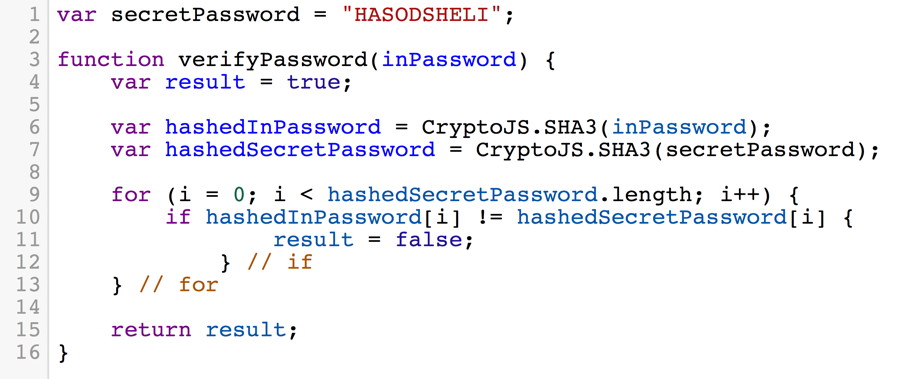
\includegraphics[scale=0.6]{images/chapter_1/password_check_algo_3.png}
    \caption{Secure password checking using a secure hash function}
    \label{c1_fig_pass_check_3}
\end{figure}

The right way to store passwords is with hashing (storing the hash of the password
rather than the password in plain text). A hash is a cryptographic function which has the property called "The Avalanche Property" which means
if even 1 bit is fliped in the input, at least half of the bits of the output are flipped as a result.
This means that even if my guess is really close to the password (1 bit away from the real password) I cannot really know which bits are correct and which are not due to the Avalanche property.

Using hashes to perform a secure password check is described in the algorithm in figure \ref{c1_fig_pass_check_3}
A guess is being hashed before it is compared against the hash of the true password.
An attacker might use the same methods from before to try to leak the hash of the true password, 
 but that would be very difficult as the attacker does not input the hash, the attacker only controls a string that is later being hashed by the algorithm.
 So the trying the methods from before to leak the password would not work if the hash used is propely implemented. 

A possible leak that can occur from this method is the length of the true password.
In line 7 of the algorithm in figure \ref{c1_fig_pass_check_3} the hash of the true password is computed.
Line 7 makes the total run time of the program dependant of the length of the true password.
While this might be risky, this is easy to fix - we can just precompute the hash of the true password
and use it whenever the algorithm runs. This is done for example in Linux where the hashes 
of user's passwords are stored in a file in \lstinline{/etc/shadow}.


\section{The Algebra Behind RSA}
The next thing we're going to perform a timing attack on is the RSA crypto system.
But before we delve into how we break RSA (next chapter) we're going to discuss the
algebraic foundation of RSA \cite{kaliski2006mathematics}.

The RSA cryptosystem lives in something called a multiplicative group.
The group that is $Z^{*}_n$.

We're taking 2 random prime numbers; $p$, $q$ and assign $n=pq$. The group $Z^{*}_n$ 
contains all the numbers from 1 to $n-1$ which do not divide $n$ (that is, do not divide $p$ or $q$).
For example: for $p=3$ and $q=5$, $n= 3*5 = 15$ so $Z^{*}_n = {\{1,2,4,7,8,11,13,14\}}$.

Like all groups, this group has the associative operation which in our case is the modular multiplication,
that is because we mentioned before that this group is a multiplicative group.
The group is also closed under that operation.

The group also has an identity element, 1. Which when multiplied by another element from the group - does not change it.

The last property this group has is that every element $r$ in the group
has an inverse element $r^{-1} \in Z^{*}_n$.

Since the exponentiation is just repeated multiplication - we consider exponentiation 
to also be a closed operation under that group. Each element has an order, the order always divides $(p-1)(q-1)$ (Fermat's little theorem).
When the element is raised to the power of the order, the result of the exponentation (under the modulu of course) is 1, the identity element in the group.

It also important to note that we cannot compute $(p-1)(q-1)$ from knowing $n$

\subsection{Elementary Operations of RSA}
To use the RSA crypto system to encrypt and decrypt messages you first have to generate the infrastructure.
That is deciding on $p$ and $q$ both large prime numbers and computing $n = pq$ and $(p-1)(q-1)$ denoted as $\phi(n)$

\begin{itemize}
    \item \textbf{Choosing a public and private key pairs}
    Choose $e \in Z^{*}_{\phi(n)}$, $d \in Z^{*}_{\phi(n)}$ such that $ed = 1$ mod $\phi(n)$.
    The public key is the pair $\langle{n,e}\rangle$  and the private key pair is  $\langle{n,d}\rangle$.
    \item \textbf{To encrypt a message}
    Choose $m \in Z^{*}_n$ as your message.
    The cipher is $m^{e}$ mod $n$ = $c$
    \item \textbf{To decrypt a message}
    Since $c = m^{e}$ mod $n$, perform $c^{d}$ = $m^{ed}$ = $m^{1}$ = $m$ mod $n$
\end{itemize}

Example: Consider $p = 3$, $q = 5$. So we can compute $n = 3*5 = 15$ and $\phi(15) = 2 * 4 = 8$
Let's assume we choose $e = 3$ and $d=11$. We consider the message 2.

To encrypt, we compute $2^{3} = 8$ mod 11, Which is the cipher. And to decrypt, we're using the private key $11$ as follows: $8^{11}$ = 2 mod 15.
And now we have our message back, 2.

Since this is not a crypto course, we will not go into any much more details about the algebra behind RSA.
However it is important for us to get familiarize with the basics of RSA in order to understand later
how it was optimized and how can we break it.

\subsection{See also}
\begin{enumerate}
    \item John Wiley and Sons Chichester , "Overview about Attacks on Smart Cards by Wolfgang Rankl, Munich", 3rd edition at John Wiley and Sons in September 2003.
    \item Thomas Popp, "An Introduction to Implementation Attacks and Countermeasures", Graz University of Technology, Institute for Applied Information Processing and Communications (IAIK) Graz, Austria.
\end{enumerate}